\documentclass[a4paper,UTF8]{ctexart}

\usepackage{amsmath, amsthm, amssymb, amsfonts, hyperref, mathrsfs}%美国数学学会的包+?
\usepackage{geometry} %控制界面
\usepackage{bookmark}
\usepackage{fancyhdr} % header & footer
\usepackage{appendix} % 附录
\usepackage{tikz} %作图
\usepackage{graphicx} %插入图片的宏包
\usepackage{float} %设置图片浮动位置的宏包
%\usepackage{subfigure} %插入多图时用子图显示的宏包
\usepackage{listings} %引用代码
\usepackage{physics,mathtools} %物理数学工具
\usepackage{comment}
\usepackage{framed}
\usepackage{caption}
\usepackage{subcaption}
\geometry{top=2.5cm,bottom=2.5cm,left=2.5cm,right=2.5cm} % 布局要求
\pagestyle{fancy} % fancy分格
\fancyhf{} % 清除所有页眉页脚
\renewcommand\headrulewidth{0.6pt}
\renewcommand\footrulewidth{0.6pt}
% font
\setCJKmainfont{Noto Serif CJK SC}[BoldFont={Noto Serif CJK SC Bold}, ItalicFont=]
\lhead{何金铭 PB21020660$\mid$座位号:6}
\cfoot{非线性光学二次谐波产生实验报告}
\rhead{\thepage}
\lfoot{2024.4.10}
\rfoot{USTC}
%\bibliographystyle{plain} % 引用样式
\everymath{\displaystyle} % display
%============================================================

\begin{document}

\begin{center}
    \textbf{\Large 非线性光学二次谐波产生实验报告}
    \par \text{\large 何金铭 PB21020660}
\end{center}

实验目的,实验原理,实验内容均于预习报告中给出,此报告不再赘述。

\section{实验结果与分析}

\subsection{II型PPKTP晶体的倍频功率与晶体温度的关系}

\begin{table}[H]
    \centering
    \caption{II型PPKTP晶体的倍频功率与晶体温度的关系记录表}
    \begin{tabular}{|l|l|l|l|}
    \hline
        晶体温度℃ & 倍频功率(mW) & 晶体温度℃ & 倍频功率(mW) \\ \hline
        33.5 & 0.25 & 39 & 4.81 \\ \hline
        34 & 0.36 & 39.5 & 3.65 \\ \hline
        34.5 & 0.43 & 40 & 2.55 \\ \hline
        35 & 0.72 & 40.5 & 1.51 \\ \hline
        35.5 & 1.65 & 41 & 0.73 \\ \hline
        36 & 2.53 & 41.5 & 0.246 \\ \hline
        36.5 & 3.78 & 42 & 0.09 \\ \hline
        37 & 4.79 & 42.5 & 0.09 \\ \hline
        37.5 & 5.56 & 43 & 0.142 \\ \hline
        38 & 5.83 & 43.5 & 0.207 \\ \hline
        38.5 & 5.56 & &\\ \hline
    \end{tabular}
\end{table}

给出了II型PPKTP晶体的倍频功率与晶体温度的关系图,如下图所示:

\begin{figure}[H]
    \centering
    \begin{minipage}[b]{0.9\textwidth}
        \centering
        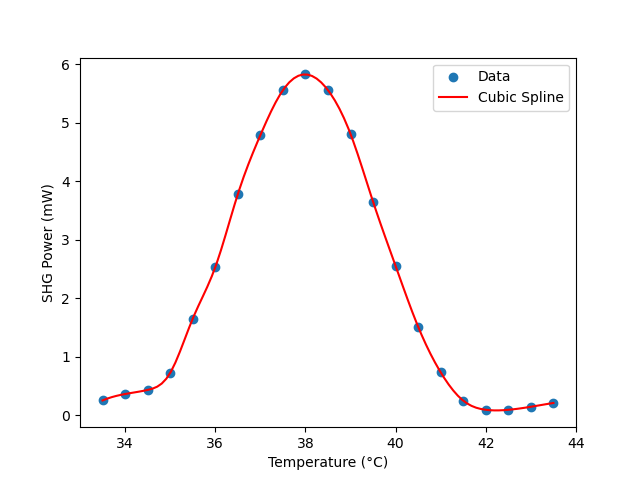
\includegraphics[width=0.8\textwidth]{./ffig1.png}
        \caption{II型PPKTP晶体的倍频功率与晶体温度的关系}
    \end{minipage}
\end{figure}

发现大致符合相位匹配中的Sinc函数平方的形状

\subsection{倍频光输出功率与基频光功率之间的关系}

此时调节晶体温度为38℃,记录了倍频光输出功率与基频光功率之间的关系,如下表所示:

\begin{table}[H]
    \centering
    \caption{倍频光输出功率与基频光功率之间的关系记录表}
    \begin{tabular}{|l|l|}
    \hline
        基频功率(mW) & 倍频功率(mW) \\ \hline
        1006 & 5.94 \\ \hline
        805 & 3.72 \\ \hline
        598 & 2.02 \\ \hline
        402 & 0.872 \\ \hline
        201 & 0.19 \\ \hline
    \end{tabular}
\end{table}

\begin{figure}[H]
    \centering
    \begin{minipage}[b]{0.9\textwidth}
        \centering
        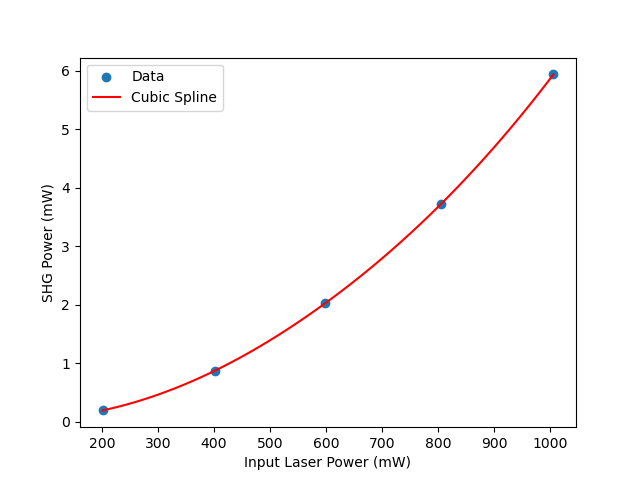
\includegraphics[width=0.8\textwidth]{./ffig2.png}
        \caption{倍频光输出功率与基频光功率之间的关系}
    \end{minipage}
\end{figure}

可以看出倍频输出功率是基频光输入功率的二次方关系

\section{实验结论}

\begin{enumerate}
    \item 测得了II型PPKTP晶体的倍频功率与晶体温度的关系,发现大致符合相位匹配中的Sinc函数平方的形状
    \item 测得了倍频光输出功率与基频光功率之间的关系,发现倍频输出功率是基频光输入功率的二次方关系
\end{enumerate}

\section{思考题}

\subsection{倍频功率与哪些因素有关?倍频功率与基频光功率是什么关系?}

倍频功率与以下因素有关:
\begin{enumerate}
    \item 基频光功率:倍频过程是将基频光转换为倍频光的过程,因此倍频功率与基频光功率密切相关。通常情况下,倍频功率随着基频光功率的增加而增加。
    \item II型PPKTP晶体的晶体温度
    \item 非线性系数:倍频过程是一个非线性光学过程,倍频功率与材料的非线性系数有关。非线性系数越大,倍频功率的转换效率就越高。
    \item 光束的空间和时间特性:光束的空间和时间特性可以影响倍频过程的效率。例如,光束的空间模式和聚焦性质可能会影响倍频功率的转换效率。
    \item 光束的偏振状态:光束的偏振状态对倍频过程也有影响。某些倍频过程对特定的偏振状态更加敏感,因此偏振状态的选择可以影响倍频功率的产生。
\end{enumerate}

\begin{align}
P_{SH}=\Bigg(\frac{2\omega_{F}^{2}d_{eff}^{2}k_{F}P_{F}^{2}}{\pi n_{F}^{2}n_{SH}\varepsilon_{0}c^{3}}\Bigg)Lh(B,\zeta), \\
\zeta=L/b,\quad b=2\pi n_F\omega_0^2/\lambda_F 
\end{align}

倍频输出功率是基频光输入功率的二次方关系。

\subsection{如何计算指定波长PPKTP晶体下I类准相位匹配在倍频转换中的极化周期?试计算780nm到390nm倍频的极化周期。}

I型位相匹配的极化周期为:

\begin{equation}
    \Lambda^{I} = \frac{\lambda_F}{2(n_{SHG}-n_{F})}
\end{equation}

在这里,$n_F$和$n_{SHG}$为基频与倍频光在晶体$z$轴方向的折射率。

对于PPKTP(铌酸锂钾盐晶体)来说,可以采用以下参数:
$λ_{F} = 780 nm$,
$n_{F} = 1.834$(对应于780 nm的折射率),
$n_{SHG} = 1.822$(对应于390 nm的折射率)。

代入计算即可

\subsection{准相位匹配中倍频功率与温度是什么关系?如何测量倍频中的温度带宽?}

准相位匹配中倍频功率与温度的关系:

\begin{equation}
    P_{SHG} \propto sinc^{2}(\frac{\Delta k L}{2})
\end{equation}

这里$\Delta k$依赖于晶体的温度以及基频光的波长。

当基频光的波长固定时,倍频的温度接收带宽为:

\begin{equation}
    \Delta T_{FWHM} = \frac{0.4429\pi}{L}\abs{\alpha(n_{SHG}-n_{F})- \frac{\partial n_F}{\partial T}\big{|}_{T=T_0} + \frac{\partial n_{SHG}}{\partial T}\big{|}_{T=T_0}}^{-1}
\end{equation}

公式中$\alpha$是材料的热膨胀系数,$T_0$表示某一特定的位相匹配温度。

测量倍频中的温度带宽通常可以采用以下方法:\

\begin{enumerate}
    \item 温度扫描法:通过改变晶体的温度,在不同温度下测量倍频功率的变化。可以绘制倍频功率与温度之间的关系曲线,从而确定倍频的温度带宽。
    \item 温度控制法:通过控制晶体的温度在一定范围内变化,并在不同温度下测量倍频功率。可以记录倍频功率随温度变化的数据,并分析其带宽范围。温度稳定性测试:在一定温度范围内保持晶体温度恒定,并测量倍频功率的稳定性。观察倍频功率的变化情况,可以推测温度带宽的范围。
    \item 温度稳定性测试:在一定温度范围内保持晶体温度恒定,并测量倍频功率的稳定性。观察倍频功率的变化情况,可以推测温度带宽的范围。
\end{enumerate}

\subsection{单次通过下的倍频转换效率较低,有哪些办法可以提升倍频的功率转换效率?}

要提高单次通过下的倍频转换效率,可以采取以下办法:

\begin{enumerate}
    \item 使用非线性光学晶体:选择具有较高非线性系数的光学晶体,例如铌酸锂(LiNbO3)、铌酸锂钾盐(PPKTP)等。这些晶体具有较高的倍频转换效率,可以提高倍频功率的产生。优化相位匹配条件:准确控制泵浦光和倍频光的相位匹配条件,使其在晶体中达到最佳匹配。可以通过调整入射角度、温度等参数来实现相位匹配的优化。
    \item 优化相位匹配条件:准确控制泵浦光和倍频光的相位匹配条件,使其在晶体中达到最佳匹配。可以通过调整入射角度、温度等参数来实现相位匹配的优化。
    \item 使用光学腔:将倍频晶体放置在光学腔中,利用光腔的谐振增强效应,提高倍频转换效率。光学腔可以增加光场与晶体的相互作用长度,增强倍频过程中的能量耦合。使用调制技术:引入调制技术,如电光调制、声光调制等,可以调制泵浦光的强度或相位,从而优化倍频转换过程,提高转换效率。
    \item 使用调制技术:引入调制技术,如电光调制、声光调制等,可以调制泵浦光的强度或相位,从而优化倍频转换过程,提高转换效率。
    \item 优化光束质量:采取合适的光束整形和聚焦手段,优化泵浦光和倍频光的光束质量,减小光束的空间展宽和相位畸变,有助于提高倍频转换效率。使用波导结构:在光学波导中进行倍频转换,可以实现较长的倍频过程长度和较高的能量耦合效率,提高转换效率。
    \item 使用波导结构:在光学波导中进行倍频转换,可以实现较长的倍频过程长度和较高的能量耦合效率,提高转换效率。
\end{enumerate}

\end{document}